\DeclareUnicodeCharacter{041B}{\CYRL}



\documentclass[11pt]{article}

    
    \usepackage{anyfontsize}
    \usepackage[breakable]{tcolorbox}
    \usepackage{parskip} % Stop auto-indenting (to mimic markdown behaviour)
    \usepackage[english,russian]{babel}
    \usepackage{graphicx}
    \usepackage{subcaption}

    % Basic figure setup, for now with no caption control since it's done
    % automatically by Pandoc (which extracts ![](path) syntax from Markdown).
    \usepackage{graphicx}
    % Maintain compatibility with old templates. Remove in nbconvert 6.0
    \let\Oldincludegraphics\includegraphics
    % Ensure that by default, figures have no caption (until we provide a
    % proper Figure object with a Caption API and a way to capture that
    % in the conversion process - todo).
    \usepackage{caption}

    \usepackage{float}
    \floatplacement{figure}{H} % forces figures to be placed at the correct location
    \usepackage{xcolor} % Allow colors to be defined
    \usepackage{enumerate} % Needed for markdown enumerations to work
    \usepackage{geometry} % Used to adjust the document margins
    \usepackage{amsmath} % Equations
    \usepackage{amssymb} % Equations
    \usepackage{textcomp} % defines textquotesingle
    % Hack from http://tex.stackexchange.com/a/47451/13684:
    \AtBeginDocument{%
        \def\PYZsq{\textquotesingle}% Upright quotes in Pygmentized code
    }
    \usepackage{upquote} % Upright quotes for verbatim code
    \usepackage{eurosym} % defines \euro

    \usepackage{iftex}
    \ifPDFTeX
        \usepackage[T1]{fontenc}
        \IfFileExists{alphabeta.sty}{
              \usepackage{alphabeta}
          }{
              \usepackage[mathletters]{ucs}
              \usepackage[utf8x]{inputenc}
          }
    \else
        \usepackage{fontspec}
        \usepackage{unicode-math}
    \fi

    \usepackage{fancyvrb} % verbatim replacement that allows latex
    \usepackage{grffile} % extends the file name processing of package graphics
                         % to support a larger range
    \makeatletter % fix for old versions of grffile with XeLaTeX
    \@ifpackagelater{grffile}{2019/11/01}
    {
      % Do nothing on new versions
    }
    {
      \def\Gread@@xetex#1{%
        \IfFileExists{"\Gin@base".bb}%
        {\Gread@eps{\Gin@base.bb}}%
        {\Gread@@xetex@aux#1}%
      }
    }
    \makeatother
    \usepackage[Export]{adjustbox} % Used to constrain images to a maximum size
    \adjustboxset{max size={0.9\linewidth}{0.9\paperheight}}

    % The hyperref package gives us a pdf with properly built
    % internal navigation ('pdf bookmarks' for the table of contents,
    % internal cross-reference links, web links for URLs, etc.)
    \usepackage{hyperref}
    % The default LaTeX title has an obnoxious amount of whitespace. By default,
    % titling removes some of it. It also provides customization options.
    \usepackage{titling}
    \usepackage{longtable} % longtable support required by pandoc >1.10
    \usepackage{booktabs}  % table support for pandoc > 1.12.2
    \usepackage{array}     % table support for pandoc >= 2.11.3
    \usepackage{calc}      % table minipage width calculation for pandoc >= 2.11.1
    \usepackage[inline]{enumitem} % IRkernel/repr support (it uses the enumerate* environment)
    \usepackage[normalem]{ulem} % ulem is needed to support strikethroughs (\sout)
                                % normalem makes italics be italics, not underlines
    \usepackage{mathrsfs}
    

    
    % Colors for the hyperref package
    \definecolor{urlcolor}{rgb}{0,.145,.698}
    \definecolor{linkcolor}{rgb}{.71,0.21,0.01}
    \definecolor{citecolor}{rgb}{.12,.54,.11}

    % ANSI colors
    \definecolor{ansi-black}{HTML}{3E424D}
    \definecolor{ansi-black-intense}{HTML}{282C36}
    \definecolor{ansi-red}{HTML}{E75C58}
    \definecolor{ansi-red-intense}{HTML}{B22B31}
    \definecolor{ansi-green}{HTML}{00A250}
    \definecolor{ansi-green-intense}{HTML}{007427}
    \definecolor{ansi-yellow}{HTML}{DDB62B}
    \definecolor{ansi-yellow-intense}{HTML}{B27D12}
    \definecolor{ansi-blue}{HTML}{208FFB}
    \definecolor{ansi-blue-intense}{HTML}{0065CA}
    \definecolor{ansi-magenta}{HTML}{D160C4}
    \definecolor{ansi-magenta-intense}{HTML}{A03196}
    \definecolor{ansi-cyan}{HTML}{60C6C8}
    \definecolor{ansi-cyan-intense}{HTML}{258F8F}
    \definecolor{ansi-white}{HTML}{C5C1B4}
    \definecolor{ansi-white-intense}{HTML}{A1A6B2}
    \definecolor{ansi-default-inverse-fg}{HTML}{FFFFFF}
    \definecolor{ansi-default-inverse-bg}{HTML}{000000}

    % common color for the border for error outputs.
    \definecolor{outerrorbackground}{HTML}{FFDFDF}

    % commands and environments needed by pandoc snippets
    % extracted from the output of `pandoc -s`
    \providecommand{\tightlist}{%
      \setlength{\itemsep}{0pt}\setlength{\parskip}{0pt}}
    \DefineVerbatimEnvironment{Highlighting}{Verbatim}{commandchars=\\\{\}}
    % Add ',fontsize=\small' for more characters per line
    \newenvironment{Shaded}{}{}
    \newcommand{\KeywordTok}[1]{\textcolor[rgb]{0.00,0.44,0.13}{\textbf{{#1}}}}
    \newcommand{\DataTypeTok}[1]{\textcolor[rgb]{0.56,0.13,0.00}{{#1}}}
    \newcommand{\DecValTok}[1]{\textcolor[rgb]{0.25,0.63,0.44}{{#1}}}
    \newcommand{\BaseNTok}[1]{\textcolor[rgb]{0.25,0.63,0.44}{{#1}}}
    \newcommand{\FloatTok}[1]{\textcolor[rgb]{0.25,0.63,0.44}{{#1}}}
    \newcommand{\CharTok}[1]{\textcolor[rgb]{0.25,0.44,0.63}{{#1}}}
    \newcommand{\StringTok}[1]{\textcolor[rgb]{0.25,0.44,0.63}{{#1}}}
    \newcommand{\CommentTok}[1]{\textcolor[rgb]{0.38,0.63,0.69}{\textit{{#1}}}}
    \newcommand{\OtherTok}[1]{\textcolor[rgb]{0.00,0.44,0.13}{{#1}}}
    \newcommand{\AlertTok}[1]{\textcolor[rgb]{1.00,0.00,0.00}{\textbf{{#1}}}}
    \newcommand{\FunctionTok}[1]{\textcolor[rgb]{0.02,0.16,0.49}{{#1}}}
    \newcommand{\RegionMarkerTok}[1]{{#1}}
    \newcommand{\ErrorTok}[1]{\textcolor[rgb]{1.00,0.00,0.00}{\textbf{{#1}}}}
    \newcommand{\NormalTok}[1]{{#1}}

    % Additional commands for more recent versions of Pandoc
    \newcommand{\ConstantTok}[1]{\textcolor[rgb]{0.53,0.00,0.00}{{#1}}}
    \newcommand{\SpecialCharTok}[1]{\textcolor[rgb]{0.25,0.44,0.63}{{#1}}}
    \newcommand{\VerbatimStringTok}[1]{\textcolor[rgb]{0.25,0.44,0.63}{{#1}}}
    \newcommand{\SpecialStringTok}[1]{\textcolor[rgb]{0.73,0.40,0.53}{{#1}}}
    \newcommand{\ImportTok}[1]{{#1}}
    \newcommand{\DocumentationTok}[1]{\textcolor[rgb]{0.73,0.13,0.13}{\textit{{#1}}}}
    \newcommand{\AnnotationTok}[1]{\textcolor[rgb]{0.38,0.63,0.69}{\textbf{\textit{{#1}}}}}
    \newcommand{\CommentVarTok}[1]{\textcolor[rgb]{0.38,0.63,0.69}{\textbf{\textit{{#1}}}}}
    \newcommand{\VariableTok}[1]{\textcolor[rgb]{0.10,0.09,0.49}{{#1}}}
    \newcommand{\ControlFlowTok}[1]{\textcolor[rgb]{0.00,0.44,0.13}{\textbf{{#1}}}}
    \newcommand{\OperatorTok}[1]{\textcolor[rgb]{0.40,0.40,0.40}{{#1}}}
    \newcommand{\BuiltInTok}[1]{{#1}}
    \newcommand{\ExtensionTok}[1]{{#1}}
    \newcommand{\PreprocessorTok}[1]{\textcolor[rgb]{0.74,0.48,0.00}{{#1}}}
    \newcommand{\AttributeTok}[1]{\textcolor[rgb]{0.49,0.56,0.16}{{#1}}}
    \newcommand{\InformationTok}[1]{\textcolor[rgb]{0.38,0.63,0.69}{\textbf{\textit{{#1}}}}}
    \newcommand{\WarningTok}[1]{\textcolor[rgb]{0.38,0.63,0.69}{\textbf{\textit{{#1}}}}}
    
% Pygments definitions
\makeatletter
\def\PY@reset{\let\PY@it=\relax \let\PY@bf=\relax%
    \let\PY@ul=\relax \let\PY@tc=\relax%
    \let\PY@bc=\relax \let\PY@ff=\relax}
\def\PY@tok#1{\csname PY@tok@#1\endcsname}
\def\PY@toks#1+{\ifx\relax#1\empty\else%
    \PY@tok{#1}\expandafter\PY@toks\fi}
\def\PY@do#1{\PY@bc{\PY@tc{\PY@ul{%
    \PY@it{\PY@bf{\PY@ff{#1}}}}}}}
\def\PY#1#2{\PY@reset\PY@toks#1+\relax+\PY@do{#2}}

\@namedef{PY@tok@w}{\def\PY@tc##1{\textcolor[rgb]{0.73,0.73,0.73}{##1}}}
\@namedef{PY@tok@c}{\let\PY@it=\textit\def\PY@tc##1{\textcolor[rgb]{0.24,0.48,0.48}{##1}}}
\@namedef{PY@tok@cp}{\def\PY@tc##1{\textcolor[rgb]{0.61,0.40,0.00}{##1}}}
\@namedef{PY@tok@k}{\let\PY@bf=\textbf\def\PY@tc##1{\textcolor[rgb]{0.00,0.50,0.00}{##1}}}
\@namedef{PY@tok@kp}{\def\PY@tc##1{\textcolor[rgb]{0.00,0.50,0.00}{##1}}}
\@namedef{PY@tok@kt}{\def\PY@tc##1{\textcolor[rgb]{0.69,0.00,0.25}{##1}}}
\@namedef{PY@tok@o}{\def\PY@tc##1{\textcolor[rgb]{0.40,0.40,0.40}{##1}}}
\@namedef{PY@tok@ow}{\let\PY@bf=\textbf\def\PY@tc##1{\textcolor[rgb]{0.67,0.13,1.00}{##1}}}
\@namedef{PY@tok@nb}{\def\PY@tc##1{\textcolor[rgb]{0.00,0.50,0.00}{##1}}}
\@namedef{PY@tok@nf}{\def\PY@tc##1{\textcolor[rgb]{0.00,0.01,2.00}{##1}}}
\@namedef{PY@tok@nc}{\let\PY@bf=\textbf\def\PY@tc##1{\textcolor[rgb]{0.00,0.01,2.00}{##1}}}
\@namedef{PY@tok@nn}{\let\PY@bf=\textbf\def\PY@tc##1{\textcolor[rgb]{0.00,0.01,2.00}{##1}}}
\@namedef{PY@tok@ne}{\let\PY@bf=\textbf\def\PY@tc##1{\textcolor[rgb]{0.80,0.25,0.22}{##1}}}
\@namedef{PY@tok@nv}{\def\PY@tc##1{\textcolor[rgb]{0.10,0.09,0.49}{##1}}}
\@namedef{PY@tok@no}{\def\PY@tc##1{\textcolor[rgb]{0.53,0.00,0.00}{##1}}}
\@namedef{PY@tok@nl}{\def\PY@tc##1{\textcolor[rgb]{0.46,0.46,0.00}{##1}}}
\@namedef{PY@tok@ni}{\let\PY@bf=\textbf\def\PY@tc##1{\textcolor[rgb]{0.44,0.44,0.44}{##1}}}
\@namedef{PY@tok@na}{\def\PY@tc##1{\textcolor[rgb]{0.41,0.47,0.13}{##1}}}
\@namedef{PY@tok@nt}{\let\PY@bf=\textbf\def\PY@tc##1{\textcolor[rgb]{0.00,0.50,0.00}{##1}}}
\@namedef{PY@tok@nd}{\def\PY@tc##1{\textcolor[rgb]{0.67,0.13,1.00}{##1}}}
\@namedef{PY@tok@s}{\def\PY@tc##1{\textcolor[rgb]{0.73,0.13,0.13}{##1}}}
\@namedef{PY@tok@sd}{\let\PY@it=\textit\def\PY@tc##1{\textcolor[rgb]{0.73,0.13,0.13}{##1}}}
\@namedef{PY@tok@si}{\let\PY@bf=\textbf\def\PY@tc##1{\textcolor[rgb]{0.64,0.35,0.47}{##1}}}
\@namedef{PY@tok@se}{\let\PY@bf=\textbf\def\PY@tc##1{\textcolor[rgb]{0.67,0.36,0.12}{##1}}}
\@namedef{PY@tok@sr}{\def\PY@tc##1{\textcolor[rgb]{0.64,0.35,0.47}{##1}}}
\@namedef{PY@tok@ss}{\def\PY@tc##1{\textcolor[rgb]{0.10,0.09,0.49}{##1}}}
\@namedef{PY@tok@sx}{\def\PY@tc##1{\textcolor[rgb]{0.00,0.50,0.00}{##1}}}
\@namedef{PY@tok@m}{\def\PY@tc##1{\textcolor[rgb]{0.40,0.40,0.40}{##1}}}
\@namedef{PY@tok@gh}{\let\PY@bf=\textbf\def\PY@tc##1{\textcolor[rgb]{0.00,0.00,0.50}{##1}}}
\@namedef{PY@tok@gu}{\let\PY@bf=\textbf\def\PY@tc##1{\textcolor[rgb]{0.50,0.00,0.50}{##1}}}
\@namedef{PY@tok@gd}{\def\PY@tc##1{\textcolor[rgb]{0.63,0.00,0.00}{##1}}}
\@namedef{PY@tok@gi}{\def\PY@tc##1{\textcolor[rgb]{0.00,0.52,0.00}{##1}}}
\@namedef{PY@tok@gr}{\def\PY@tc##1{\textcolor[rgb]{0.89,0.00,0.00}{##1}}}
\@namedef{PY@tok@ge}{\let\PY@it=\textit}
\@namedef{PY@tok@gs}{\let\PY@bf=\textbf}
\@namedef{PY@tok@gp}{\let\PY@bf=\textbf\def\PY@tc##1{\textcolor[rgb]{0.00,0.00,0.50}{##1}}}
\@namedef{PY@tok@go}{\def\PY@tc##1{\textcolor[rgb]{0.44,0.44,0.44}{##1}}}
\@namedef{PY@tok@gt}{\def\PY@tc##1{\textcolor[rgb]{0.00,0.27,0.87}{##1}}}
\@namedef{PY@tok@err}{\def\PY@bc##1{{\setlength{\fboxsep}{\string -\fboxrule}\fcolorbox[rgb]{1.00,0.00,0.00}{1,1,1}{\strut ##1}}}}
\@namedef{PY@tok@kc}{\let\PY@bf=\textbf\def\PY@tc##1{\textcolor[rgb]{0.00,0.50,0.00}{##1}}}
\@namedef{PY@tok@kd}{\let\PY@bf=\textbf\def\PY@tc##1{\textcolor[rgb]{0.00,0.50,0.00}{##1}}}
\@namedef{PY@tok@kn}{\let\PY@bf=\textbf\def\PY@tc##1{\textcolor[rgb]{0.00,0.50,0.00}{##1}}}
\@namedef{PY@tok@kr}{\let\PY@bf=\textbf\def\PY@tc##1{\textcolor[rgb]{0.00,0.50,0.00}{##1}}}
\@namedef{PY@tok@bp}{\def\PY@tc##1{\textcolor[rgb]{0.00,0.50,0.00}{##1}}}
\@namedef{PY@tok@fm}{\def\PY@tc##1{\textcolor[rgb]{0.00,0.01,2.00}{##1}}}
\@namedef{PY@tok@vc}{\def\PY@tc##1{\textcolor[rgb]{0.10,0.09,0.49}{##1}}}
\@namedef{PY@tok@vg}{\def\PY@tc##1{\textcolor[rgb]{0.10,0.09,0.49}{##1}}}
\@namedef{PY@tok@vi}{\def\PY@tc##1{\textcolor[rgb]{0.10,0.09,0.49}{##1}}}
\@namedef{PY@tok@vm}{\def\PY@tc##1{\textcolor[rgb]{0.10,0.09,0.49}{##1}}}
\@namedef{PY@tok@sa}{\def\PY@tc##1{\textcolor[rgb]{0.73,0.13,0.13}{##1}}}
\@namedef{PY@tok@sb}{\def\PY@tc##1{\textcolor[rgb]{0.73,0.13,0.13}{##1}}}
\@namedef{PY@tok@sc}{\def\PY@tc##1{\textcolor[rgb]{0.73,0.13,0.13}{##1}}}
\@namedef{PY@tok@dl}{\def\PY@tc##1{\textcolor[rgb]{0.73,0.13,0.13}{##1}}}
\@namedef{PY@tok@s2}{\def\PY@tc##1{\textcolor[rgb]{0.73,0.13,0.13}{##1}}}
\@namedef{PY@tok@sh}{\def\PY@tc##1{\textcolor[rgb]{0.73,0.13,0.13}{##1}}}
\@namedef{PY@tok@s1}{\def\PY@tc##1{\textcolor[rgb]{0.73,0.13,0.13}{##1}}}
\@namedef{PY@tok@mb}{\def\PY@tc##1{\textcolor[rgb]{0.40,0.40,0.40}{##1}}}
\@namedef{PY@tok@mf}{\def\PY@tc##1{\textcolor[rgb]{0.40,0.40,0.40}{##1}}}
\@namedef{PY@tok@mh}{\def\PY@tc##1{\textcolor[rgb]{0.40,0.40,0.40}{##1}}}
\@namedef{PY@tok@mi}{\def\PY@tc##1{\textcolor[rgb]{0.40,0.40,0.40}{##1}}}
\@namedef{PY@tok@il}{\def\PY@tc##1{\textcolor[rgb]{0.40,0.40,0.40}{##1}}}
\@namedef{PY@tok@mo}{\def\PY@tc##1{\textcolor[rgb]{0.40,0.40,0.40}{##1}}}
\@namedef{PY@tok@ch}{\let\PY@it=\textit\def\PY@tc##1{\textcolor[rgb]{0.24,0.48,0.48}{##1}}}
\@namedef{PY@tok@cm}{\let\PY@it=\textit\def\PY@tc##1{\textcolor[rgb]{0.24,0.48,0.48}{##1}}}
\@namedef{PY@tok@cpf}{\let\PY@it=\textit\def\PY@tc##1{\textcolor[rgb]{0.24,0.48,0.48}{##1}}}
\@namedef{PY@tok@c1}{\let\PY@it=\textit\def\PY@tc##1{\textcolor[rgb]{0.24,0.48,0.48}{##1}}}
\@namedef{PY@tok@cs}{\let\PY@it=\textit\def\PY@tc##1{\textcolor[rgb]{0.24,0.48,0.48}{##1}}}

\def\PYZbs{\char`\\}
\def\PYZus{\char`\_}
\def\PYZob{\char`\{}
\def\PYZcb{\char`\}}
\def\PYZca{\char`\^}
\def\PYZam{\char`\&}
\def\PYZlt{\char`\<}
\def\PYZgt{\char`\>}
\def\PYZsh{\char`\#}
\def\PYZpc{\char`\%}
\def\PYZdl{\char`\$}
\def\PYZhy{\char`\-}
\def\PYZsq{\char`\'}
\def\PYZdq{\char`\"}
\def\PYZti{\char`\~}
% for compatibility with earlier versions
\def\PYZat{@}
\def\PYZlb{[}
\def\PYZrb{]}
\makeatother


    % For linebreaks inside Verbatim environment from package fancyvrb.
    \makeatletter
        \newbox\Wrappedcontinuationbox
        \newbox\Wrappedvisiblespacebox
        \newcommand*\Wrappedvisiblespace {\textcolor{red}{\textvisiblespace}}
        \newcommand*\Wrappedcontinuationsymbol {\textcolor{red}{\llap{\tiny$\m@th\hookrightarrow$}}}
        \newcommand*\Wrappedcontinuationindent {3ex }
        \newcommand*\Wrappedafterbreak {\kern\Wrappedcontinuationindent\copy\Wrappedcontinuationbox}
        % Take advantage of the already applied Pygments mark-up to insert
        % potential linebreaks for TeX processing.
        %        {, <, #, %, $, ' and ": go to next line.
        %        _, }, ^, &, >, - and ~: stay at end of broken line.
        % Use of \textquotesingle for straight quote.
        \newcommand*\Wrappedbreaksatspecials {%
            \def\PYGZus{\discretionary{\char`\_}{\Wrappedafterbreak}{\char`\_}}%
            \def\PYGZob{\discretionary{}{\Wrappedafterbreak\char`\{}{\char`\{}}%
            \def\PYGZcb{\discretionary{\char`\}}{\Wrappedafterbreak}{\char`\}}}%
            \def\PYGZca{\discretionary{\char`\^}{\Wrappedafterbreak}{\char`\^}}%
            \def\PYGZam{\discretionary{\char`\&}{\Wrappedafterbreak}{\char`\&}}%
            \def\PYGZlt{\discretionary{}{\Wrappedafterbreak\char`\<}{\char`\<}}%
            \def\PYGZgt{\discretionary{\char`\>}{\Wrappedafterbreak}{\char`\>}}%
            \def\PYGZsh{\discretionary{}{\Wrappedafterbreak\char`\#}{\char`\#}}%
            \def\PYGZpc{\discretionary{}{\Wrappedafterbreak\char`\%}{\char`\%}}%
            \def\PYGZdl{\discretionary{}{\Wrappedafterbreak\char`\$}{\char`\$}}%
            \def\PYGZhy{\discretionary{\char`\-}{\Wrappedafterbreak}{\char`\-}}%
            \def\PYGZsq{\discretionary{}{\Wrappedafterbreak\textquotesingle}{\textquotesingle}}%
            \def\PYGZdq{\discretionary{}{\Wrappedafterbreak\char`\"}{\char`\"}}%
            \def\PYGZti{\discretionary{\char`\~}{\Wrappedafterbreak}{\char`\~}}%
        }
        % Some characters . , ; ? ! / are not pygmentized.
        % This macro makes them "active" and they will insert potential linebreaks
        \newcommand*\Wrappedbreaksatpunct {%
            \lccode`\~`\.\lowercase{\def~}{\discretionary{\hbox{\char`\.}}{\Wrappedafterbreak}{\hbox{\char`\.}}}%
            \lccode`\~`\,\lowercase{\def~}{\discretionary{\hbox{\char`\,}}{\Wrappedafterbreak}{\hbox{\char`\,}}}%
            \lccode`\~`\;\lowercase{\def~}{\discretionary{\hbox{\char`\;}}{\Wrappedafterbreak}{\hbox{\char`\;}}}%
            \lccode`\~`\:\lowercase{\def~}{\discretionary{\hbox{\char`\:}}{\Wrappedafterbreak}{\hbox{\char`\:}}}%
            \lccode`\~`\?\lowercase{\def~}{\discretionary{\hbox{\char`\?}}{\Wrappedafterbreak}{\hbox{\char`\?}}}%
            \lccode`\~`\!\lowercase{\def~}{\discretionary{\hbox{\char`\!}}{\Wrappedafterbreak}{\hbox{\char`\!}}}%
            \lccode`\~`\/\lowercase{\def~}{\discretionary{\hbox{\char`\/}}{\Wrappedafterbreak}{\hbox{\char`\/}}}%
            \catcode`\.\active
            \catcode`\,\active
            \catcode`\;\active
            \catcode`\:\active
            \catcode`\?\active
            \catcode`\!\active
            \catcode`\/\active
            \lccode`\~`\~
        }
    \makeatother

    \let\OriginalVerbatim=\Verbatim
    \makeatletter
    \renewcommand{\Verbatim}[1][1]{%
        %\parskip\z@skip
        \sbox\Wrappedcontinuationbox {\Wrappedcontinuationsymbol}%
        \sbox\Wrappedvisiblespacebox {\FV@SetupFont\Wrappedvisiblespace}%
        \def\FancyVerbFormatLine ##1{\hsize\linewidth
            \vtop{\raggedright\hyphenpenalty\z@\exhyphenpenalty\z@
                \doublehyphendemerits\z@\finalhyphendemerits\z@
                \strut ##1\strut}%
        }%
        % If the linebreak is at a space, the latter will be displayed as visible
        % space at end of first line, and a continuation symbol starts next line.
        % Stretch/shrink are however usually zero for typewriter font.
        \def\FV@Space {%
            \nobreak\hskip\z@ plus\fontdimen3\font minus\fontdimen4\font
            \discretionary{\copy\Wrappedvisiblespacebox}{\Wrappedafterbreak}
            {\kern\fontdimen2\font}%
        }%

        % Allow breaks at special characters using \PYG... macros.
        \Wrappedbreaksatspecials
        % Breaks at punctuation characters . , ; ? ! and / need catcode=\active
        \OriginalVerbatim[#1,codes*=\Wrappedbreaksatpunct]%
    }
    \makeatother

    % Exact colors from NB
    \definecolor{incolor}{HTML}{303F9F}
    \definecolor{outcolor}{HTML}{D84315}
    \definecolor{cellborder}{HTML}{CFCFCF}
    \definecolor{cellbackground}{HTML}{F7F7F7}

    % prompt
    \makeatletter
    \newcommand{\boxspacing}{\kern\kvtcb@left@rule\kern\kvtcb@boxsep}
    \makeatother
    \newcommand{\prompt}[4]{
        {\ttfamily\llap{{\color{#2}[#3]:\hspace{3pt}#4}}\vspace{-\baselineskip}}
    }
    

    
    % Prevent overflowing lines due to hard-to-break entities
    \sloppy
    % Setup hyperref package
    \hypersetup{
      breaklinks=true,  % so long urls are correctly broken across lines
      colorlinks=true,
      urlcolor=urlcolor,
      linkcolor=linkcolor,
      citecolor=citecolor,
      }
    % Slightly bigger margins than the latex defaults
    
    \geometry{verbose,tmargin=1in,bmargin=1in,lmargin=1in,rmargin=1in}
    
    

\begin{document}

    \begin{titlepage}
    \newpage
    
    \begin{center}
    МИНИСТЕРСТВО ОБРАЗОВАНИЯ РЕСПУБЛИКИ БЕЛАРУСЬ БЕЛОРУССКИЙ ГОСУДАРСТВЕННЫЙ УНИВЕРСИТЕТ \\
    Факультет прикладной математики и информатики \\ Кафедра компьютерных технологий и систем
    \end{center}
    
    \vspace{8em}
    
    \vspace{2em}
    
    \begin{center}
    \textsc{\textbf{Отчет по лабораторной работе 3
    \linebreak Вариант 2}}
    \end{center}
    
    \vspace{6em}
    
    \begin{flushright}
        Выполнил:\\
        Карпович Артём Дмитриевич\\
        студент 4 курса 7 группы
    \end{flushright}

    \begin{flushright}
        Преподаватель:\\
        Каркоцкий Александр Геннадьевич
    \end{flushright}
    \vspace{\fill}
    
    \begin{center}
    Минск, 2024
    \end{center}
    
    \end{titlepage}

\begin{center}
    \section*{Условие}
\end{center}
Найти электрический и магнитный потенциал, электрическую и магнитную напряжённость внутри шара (внутри сферического слоя) при заданных диэлектрической проницаемости $\varepsilon$, условиях на электрический и магнитный потенциал ($u$ и $v$ соответственно) на его
поверхности (на границах сферического слоя), и постоянной магнитной проницаемости,
если распределение зарядов изменяется по закону $\rho(r, \varphi, \theta)$.

$$\varepsilon=3,\rho(r,\varphi,\theta)=12r^5 \cos^2(\theta)(\sin^2(\theta)\cos(2\varphi) - \sin(\theta)\sin(\varphi));$$
$$u|_{r=3}=5\cos^2(\varphi)\sin^4(\theta)\cos(\theta).$$

$$v|_{r=2}=4\sin(\varphi)\sin(\theta)\cos^2(\theta);$$
$$v|_{r=5}=6\cos^2(\varphi)\sin^2(\theta)\cos(\theta).$$
\newpage
\section*{Задача 1}
\subsubsection*{Получение решения}
Перепишем условие задачи:
$$\begin{cases}
    \Delta u=-\frac{\rho(x,y,z)}{\varepsilon}=-4r^5 \cos^2(\theta)(\sin^2(\theta)\cos(2\varphi) - \sin(\theta)\sin(\varphi)),\\
    u|_{r=3}=5\cos^2(\varphi)\sin^4(\theta)\cos(\theta).\\
\end{cases}$$

 Решение задачи ищем в виде $$u(r,\theta,\varphi)=v(r,\theta,\varphi)+\omega(r,\theta,\varphi).$$
 Функцию $v$ будем искать так, чтобы занулить граничные условия, то есть получим задачу:
 $$\begin{cases}
     \Delta v=-4r^5 \cos^2(\theta)(\sin^2(\theta)\cos(2\varphi) - \sin(\theta)\sin(\varphi)),\\
    v|_{r=3}=0.
 \end{cases}$$
 Для $\omega$ имеем задачу:
  $$\begin{cases}
     \Delta \omega=0,\\
    \omega|_{r=3}=5\cos^2(\varphi)\sin^4(\theta)\cos(\theta).
 \end{cases}$$
 Сначала решим именно эту задачу. Решение ее представимо в виде:
 $$\omega(r,\theta,\varphi)=\sum_{n,m=0}^\infty (A_{nm} \cos(m\varphi) + B_{nm} \sin(m\varphi))r^n P_n^{(m)}(\cos(\theta))$$
 Воспользуемся граничными условиями:
 $$\omega|_{r=3}=\sum_{n,m=0}^\infty (A_{nm} \cos(m\varphi) + B_{nm} \sin(m\varphi))3^n P_n^{(m)}(\cos(\theta))=5\Big( \frac{1+\cos(2\varphi)}{2} \Big)\sin^4(\theta)\cos(\theta)=$$$$=\frac{5}{2}\sin^4(\theta)\cos(\theta)\cos(0\varphi)+\frac{5}{2}\sin^4(\theta)\cos(\theta)\cos(2\varphi).$$
 Тогда:
 $$A_{nm}=\begin{cases}
     A_{n0}, m=0,\\
     A_{n2}, m=2,\\
     0, m\neq 1,
 \end{cases}\ B_{nm}=0$$
 Таким образом,
 $$\omega|_{r=3}=\sum_{n=0}^\infty (A_{n0} P_n^{(0)}(\cos(\theta))+A_{n2}\cos(2\varphi)P_n^{(2)}(\cos(\theta))3^n)=\frac{5}{2}\sin^4(\theta)\cos(\theta)\cos(0\varphi)+\frac{5}{2}\sin^4(\theta)\cos(\theta)\cos(2\varphi).$$
 Тогда получим два уравнения:
 $$\sum_{n=0}^\infty (3^nA_{n0} P_n^{(0)}(\cos(\theta))=\frac{5}{2}\sin^4(\theta)\cos(\theta),$$
 $$\sum_{n=0}^\infty (3^nA_{n2} P_n^{(2)}(\cos(\theta))=\frac{5}{2}\sin^4(\theta)\cos(\theta)$$
 Введем замену $\cos(\theta) = x$, тогда получим уравнение $$\frac{5}{2}(1-x^2)^2x=\frac{5}{2}(x^5-2x^3+x),$$ то есть имеем уравнение пятой степени. 

 Для вычисления полиномов Лежандра воспользуемся формулой:
 $$P_n^{(0)}(x)=\frac{1}{2^nn!}\frac{d^n}{dx^n}(x^2-1)^n.$$
 $$\deg P_n^{(0)}(x)=2n-n\leq5\Rightarrow n\leq5.$$
 С помощью таблицы выпишем $P_n^{(0)}, n=\overline{0,5}:$
 $$P_0^{(0)}=1,$$
 $$P_1^{(0)}=x,$$
 $$P_2^{(0)}=\frac{1}{2}(3x^2-1),$$
 $$P_3^{(0)}=\frac{1}{2}(5x^3-3x),$$
 $$P_4^{(0)}=\frac{1}{8}(35x^4-30x^2+3),$$
 $$P_5^{(0)}=\frac{1}{8}(63x^5-70x^3+15x).$$
 Подставим в первое из полученных ранее уравнений:
 $$A_{00}+3A_{10}x+\frac{9}{2}A_{20}(3x^2-1)+\frac{27}{2}A_{30}(5x^3-3x)+\frac{81}{8}A_{40}(35x^4-30x^2+3)+\frac{243}{8}A_{50}(63x^5-70x^3+15x)=$$$$=\frac{5}{2}(x^5-2x^3+x)$$
 Приравняем коэффициенты при соответствующих степенях:
 $$\begin{cases}
     A_{50}=\frac{5\cdot8}{2\cdot243\cdot63}=\frac{20}{15309},\\
     A_{40}=0,\\
     A_{30}=\frac{2}{27\cdot5}(-5+\frac{243\cdot 70}{8}A_{05})=-\frac{8}{243},\\
     A_{20}=0,\\
     A_{10}=\frac{1}{3}\Big(\frac{5}{2}+\frac{81}{2}A_{30}-\frac{243\cdot15}{8}A_{50}\Big)=\frac{4}{21},\\
     A_{00}=\frac{9}{2}A_{02}-\frac{3\cdot81}{8}A_{40}=0
 \end{cases}$$
  Аналогичным образом поступим для второго уравнения. Полиномы Лежандра в этом случае вычисляются по формуле:
 $$P_n^{(2)}(x)=\frac{1-x^2}{2^n n!}\frac{d^{n+2}}{dx^{n+2}}(x^2-1)^n,$$
 $$\deg P_n^{(2)}=2+2n-(n+2)=n\leq5.$$
 Используя таблицу, выпишем для $n=\overline{2,5}:$
 $$P_2^{(2)}(x)=3(1-x^2),$$
 $$P_3^{(2)}(x)=15x(1-x^2),$$
 $$P_4^{(2)}(x)=\frac{15}{2}(7x^2-1)(1-x^2),$$
 $$P_5^{(2)}(x)=\frac{105}{2}(3x^3-x)(1-x^2).$$
 Подставим в уравнение:
 $$(1-x^2)(9A_{22}\cdot3+27A_{32}\cdot15x+81A_{42}\frac{15}{2}(7x^2-1)+243A_{52}\frac{105}{2}(3x^3-x))=\frac{5}{2}(1-x^2)^2x,$$
 cократим на $1-x^2$:
 $$27(A_{22}+15A_{32}x+\frac{45}{2}A_{42}(7x^2-1)+\frac{945}{2}A_{52}(3x^3-x))=\frac{5}{2}(x-x^3).$$
 Найдем коэффициенты:
 $$\begin{cases}
     A_{52}=-\frac{5\cdot2}{54\cdot945\cdot3}=-\frac{1}{15309},\\
     A_{42}=0,\\
     A_{32}=\frac{1}{15}(\frac{5}{54}+\frac{945}{2}A_{52})=\frac{1}{243},\\
     A_{22}=\frac{45}{2}A_{42}=0.
 \end{cases}$$
 Таким образом, получаем:
 $$\omega(r,\theta, \varphi)=\Big(r\cdot\frac{4}{21}P_1^{(0)}(\cos(\theta))-r^3\cdot\frac{8}{243}P_3^{(0)}(\cos(\theta))+r^5\cdot\frac{20}{15309}P_5^{(0)}(\cos(\theta))\Big)\cos(0\varphi)+$$$$+\Big(r^3\cdot\frac{1}{243}P_3^{(2)}(\cos(\theta))-r^5\frac{1}{15309}P_5^{(2)}(\cos(\theta))\Big)\cos(2\varphi)$$
 Вернемся к задаче для $v$:
 $$\begin{cases}
     \Delta v=-4r^5 \cos^2(\theta)(\sin^2(\theta)\cos(2\varphi) - \sin(\theta)\sin(\varphi)),\\
    v|_{r=3}=0.
 \end{cases}$$
 По виду правой части запишем
 $$-4r^5 \cos^2(\theta)\sin^2(\theta)\cos(2\varphi) +4r^5 \cos^2(\theta) \sin(\theta)\sin(\varphi)=r^5\cos(2\varphi)\sum_{n=0}^\infty A_{n2}P_n^{(2)}(\cos(\theta))+$$$$+r^5\sin(\varphi)\sum_{n=0}^\infty B_{n1}P_n^{(1)}(\cos(\theta)).$$
 Тогда получим два уравнения:
 $$\sum_{n=0}^\infty A_{n2}P_n^{(2)}(\cos(\theta))=-4\cos^2(\theta)\sin^2(\theta),$$
 $$\sum_{n=0}^\infty B_{n1}P_n^{(1)}(\cos(\theta))=4\cos^2(\theta) \sin(\theta).$$
 Рассмотрим правую часть первого уравнения, введя замену $x=\cos(\theta):$
 $$-4x^2(1-x^2)=-4x^2+4x^4, \Rightarrow \deg P_n^{(2)}=n\leq4.$$
 Полиномы Лежандра до $n=4$ у нас уже есть, поэтому подставим их в наше уравнение:
 $$A_{22}3(1-x^2)+A_{32}15x(1-x^2)+A_{42}\frac{15}{2}(7x^2-1)(1-x^2)=-4x^2(1-x^2),$$
 сократим на $1-x^2$:
 $$3A_{22}+15A_{32}x+\frac{15}{2}A_{42}(7x^2-1)=-4x^2.$$
 Приравняем коэффициенты при соответствующих степенях:
 $$\begin{cases}
     A_{42}=-\frac{2\cdot4}{15\cdot7}=-\frac{8}{105},\\
     A_{32}=0,\\
     A_{22}=\frac{15}{2\cdot3}A_{42}=-\frac{4}{21}.
 \end{cases}$$
 Рассмотрим второе уравнение. Полиному Лежандра в этом случае считаем по формуле
 $$P_n^{(1)}(x)=\frac{(1-x^2)^\frac{1}{2}}{2^nn!}\frac{d^{n+1}}{dx^{n+1}}(x^2-1)^n=1+2n-(n+1)=n\leq \deg(x^2\sqrt{1-x^2})=3,\Rightarrow n\leq3.$$
 Воспользуемся таблицой и выпишем полиномы Лежандра для $n=\overline{1,3}:$
 $$P_1^{(1)}=(1-x^2)^\frac{1}{2},$$
 $$P_2^{(1)}=3x(1-x^2)^\frac{1}{2},$$
 $$P_3^{(1)}=\frac{3}{2}(5x^2-1)(1-x^2)^\frac{1}{2}.$$
 Подставим во второе уравнение:
 $$(1-x^2)^\frac{1}{2}(B_{11}+3B_{21}x+\frac{3}{2}B_{31}(5x^2-1))=4x^2(1-x^2)^\frac{1}{2}.$$
 Сократим на $(1-x^2)^\frac{1}{2}:$
 $$B_{11}+3B_{21}x+\frac{3}{2}B_{31}(5x^2-1)=4x^2.$$
 Приравняем коэффициенты при соответствующих степенях:
 $$\begin{cases}
     B_{31}=\frac{4\cdot2}{3\cdot5}=\frac{8}{15},\\
     B_{21}=0,\\
     B_{11}=\frac{3}{2}B_{31}=\frac{4}{5}.
 \end{cases}$$
 Таким образом, неоднородность представима в виде:
 $$r^5\cos(2\varphi)\Big(-\frac{4}{21}P_2^{(2)}(\cos(\theta))-\frac{8}{105}P_4^{(2)}(\cos(\theta))\Big)+r^5\sin(\varphi)\Big(\frac{4}{5}P_1^{(1)}(\cos(\theta))+\frac{8}{15}P_3^{(1)}(\cos(\theta))\Big)$$
 Введем замены $\cos(2\varphi)P_n^{(2)}(\cos(\theta))=Y_n^{(2)}(\theta, \varphi),$ $\sin(\varphi)P_n^{(1)}\cos(\theta)=Y_n^{(1)}(\theta, \varphi)$. Тогда неоднородность примет вид:
 $$r^5\Big( -\frac{4}{21}Y_2^{(2)}(\theta, \varphi)-\frac{8}{105}Y_4^{(2)}(\theta, \varphi)+\frac{4}{5}Y_1^{(1)}(\theta, \varphi)+\frac{8}{15}Y_3^{(1)}(\theta, \varphi)\Big)$$
 Следовательно, решение задачи ищем в виде:
 $$v(r,\theta, \varphi)=Z_1(r)Y_2^{(2)}(\theta, \varphi)+Z_2(r)Y_4^{(2)}(\theta, \varphi)+Z_3(r)Y_1^{(1)}(\theta, \varphi)+Z_4(r)Y_3^{(1)}(\theta, \varphi)$$
 Подставим данное представление в
 $$\Delta v=\frac{1}{r^2}\frac{\partial}{\partial r}(r^2v_r)+\frac{1}{r^2\sin(\theta)}\frac{\partial}{\partial \theta}(v_\theta \sin(\theta))+\frac{v_{\varphi \varphi}}{r^2 \sin^2(\theta)}=$$
 $$=\frac{1}{r^2}\Big[(2rZ_1'(r)+r^2Z_1''(r))Y_2^{(2)}+(2rZ_2'(r)+r^2Z_2''(r))Y_4^{(2)}+(2rZ_3'(r)+r^2Z_3''(r))Y_1^{(1)}+(2rZ_4'(r)+r^2Z_4''(r))Y_3^{(1)}\Big]+$$$$+
 \frac{Z_1}{r^2}\Big(\frac{1}{\sin(\theta)}\frac{\partial}{\partial \theta}((Y_2^{(2)})_\theta \sin(\theta))+\frac{(Y_2^{(2)})_{\varphi \varphi}}{\sin^2(\theta)}+6Y_2^{(2)}-6Y_2^{(2)}\Big)+$$$$
 +\frac{Z_2}{r^2}\Big(\frac{1}{\sin(\theta)}\frac{\partial}{\partial \theta}((Y_4^{(2)})_\theta \sin(\theta))+\frac{(Y_4^{(2)})_{\varphi \varphi}}{\sin^2(\theta)}+20Y_4^{(2)}-20Y_4^{(2)}\Big)+$$$$+
 \frac{Z_3}{r^2}\Big(\frac{1}{\sin(\theta)}\frac{\partial}{\partial \theta}((Y_1^{(1)})_\theta \sin(\theta))+\frac{(Y_1^{(1)})_{\varphi \varphi}}{\sin^2(\theta)}+2Y_1^{(1)}-2Y_1^{(2)}\Big)+$$$$
 +
 \frac{Z_4}{r^2}\Big(\frac{1}{\sin(\theta)}\frac{\partial}{\partial \theta}((Y_3^{(1)})_\theta \sin(\theta))+\frac{(Y_3^{(1)})_{\varphi \varphi}}{\sin^2(\theta)}+12Y_3^{(1)}-12Y_3^{(1)}\Big)=$$
 $$=r^5\Big( -\frac{4}{21}Y_2^{(2)}(\theta, \varphi)-\frac{8}{105}Y_4^{(2)}(\theta, \varphi)+\frac{4}{5}Y_1^{(1)}(\theta, \varphi)+\frac{8}{15}Y_3^{(1)}(\theta, \varphi)\Big).$$
 Поскольку мы работаем со сферическими функциями, то
 $$\Big(\frac{1}{\sin(\theta)}\frac{\partial}{\partial \theta}((Y_n^{(m)})_\theta \sin(\theta))+\frac{(Y_n^{(m)})_{\varphi \varphi}}{\sin^2(\theta)}+n(n+1)Y_n^{(m)}\Big) = 0.$$
 Таким образом, для каждого $Z_i(r), i=\overline{1,4}$ мы можем составить задачи Коши:
 $$\begin{cases}
     \frac{1}{r^2}\Big(2rZ_1'(r)+r^2Z_1''(r)-6Z_1\Big)=-r^5\frac{4}{21},\\
     Z_1(3)=0.
 \end{cases}$$
 Рассмотрим уравнение данной задачи:
 $$r^2Z_1''(r)+2rZ_1'(r)-6Z_1(r)=-\frac{4r^7}{21}$$
 Найдем общее решение однородного уравнения. Для этого будем искать решение в виде $Z_1(r) = r^k,$ тогда, подставив, получим:
 $$(k^2-k)r^k+2kr^k-6r^k=0,\Rightarrow k^2+k-6=0, \Rightarrow k_{1,2}=2, -3.$$
 Таким образом, получаем, что $$Z_1^{\text{оо}}(r)=C_1r^2.$$
 Частное решение неоднородного ищем в виде $$Z_1^{\text{чн}}(r)=Ar^7\Rightarrow42Ar^7+14Ar^7-6Ar^7=-\frac{4r^7}{21},\Rightarrow50A=-\frac{4}{21},\Rightarrow A=-\frac{2}{525}.$$
 Таким образом,
 $$Z_1^{\text{он}}(r)=C_1r^2-\frac{2}{525}r^7.$$
 Подставим начальное условие:
 $$Z_1(3)=9C_1-\frac{2\cdot 3^7}{525}=0, \Rightarrow C_1=\frac{2\cdot 3^5}{525}\Rightarrow Z_1(r) = \frac{486}{525}r^2-\frac{2}{525}r^7.$$
 Аналогичным образом найдем и остальные $Z_i(r):$
 
 $Z_2(r):$
 $$\begin{cases}
     \frac{1}{r^2}\Big(2rZ_2'(r)+r^2Z_2''(r)-20Z_2(r)\Big)=-r^5\frac{8}{105},\\
     Z_2(3)=0.
 \end{cases}$$
 $$Z_2^{\text{оо}}(r)=C_1r^4,$$
 $$Z_2^{\text{чн}}(r)=-\frac{2}{945}r^7,$$
 $$Z_2(3)=3^4C_1-\frac{2\cdot3^7}{945}=0, \Rightarrow C_1=\frac{54}{945}, \Rightarrow Z_2(r)=\frac{54}{945}r^4-\frac{2}{945}r^7.$$
 $Z_3(r):$
 $$\begin{cases}
     \frac{1}{r^2}\Big(2rZ_3'(r)+r^2Z_3''(r)-2Z_3(r)\Big)=r^5\frac{4}{5},\\
     Z_3(3)=0.
 \end{cases}$$
 $$Z_3^{\text{оо}}(r)=C_1r,$$
 $$Z_3^{\text{чн}}(r)=\frac{2}{135}r^7,$$
 $$Z_3(3)=3C_1+\frac{2\cdot3^7}{135}=0, \Rightarrow C_1=-\frac{2\cdot 3^6}{135}=-\frac{54}{5}, \Rightarrow Z_3(r)=-\frac{54}{5}r+\frac{2}{135}r^7.$$
 $Z_4(r):$
 $$\begin{cases}
     \frac{1}{r^2}\Big(2rZ_4'(r)+r^2Z_4''(r)-12Z_4(r)\Big)=r^5\frac{8}{15},\\
     Z_4(3)=0.
 \end{cases}$$
 $$Z_4^{\text{оо}}(r)=C_1r^3,$$
 $$Z_4^{\text{чн}}(r)=\frac{2}{165}r^7,$$
 $$Z_4(3)=3^3C_1+\frac{2\cdot3^7}{165}=0, \Rightarrow C_1=-\frac{54}{55}, \Rightarrow Z_4(r)=-\frac{54}{55}r^3+\frac{2}{165}r^7.$$
 Таким образом, решение рассматриваемой задачи представимо в виде:
 $$v(r,\theta, \varphi) = \Big( \frac{486}{525}r^2-\frac{2}{525}r^7 \Big)\cos(2\varphi)P_2^{(2)}(\cos(\theta))+\Big( \frac{54}{945}r^4-\frac{2}{945}r^7\Big)\cos(2\varphi)P_4^{(2)}(\cos(\theta))+$$$$+\Big(-\frac{54}{5}r+\frac{2}{135}r^7 \Big)\sin(\varphi)P_1^{(1)}\cos(\theta)+\Big(-\frac{54}{55}r^3+\frac{2}{165}r^7\Big)\sin(\varphi)P_3^{(1)}\cos(\theta).$$
 И решение исходной задачи имеет вид:
 $$u(r, \theta, \varphi) = \Big( \frac{486}{525}r^2-\frac{2}{525}r^7 \Big)\cos(2\varphi)P_2^{(2)}(\cos(\theta))+\Big( \frac{54}{945}r^4-\frac{2}{945}r^7\Big)\cos(2\varphi)P_4^{(2)}(\cos(\theta))+$$$$+\Big(-\frac{54}{5}r+\frac{2}{135}r^7 \Big)\sin(\varphi)P_1^{(1)}\cos(\theta)+\Big(-\frac{54}{55}r^3+\frac{2}{165}r^7\Big)\sin(\varphi)P_3^{(1)}\cos(\theta)+$$
 $$+\Big(r\cdot\frac{4}{21}P_1^{(0)}(\cos(\theta))-r^3\cdot\frac{8}{243}P_3^{(0)}(\cos(\theta))+r^5\cdot\frac{20}{15309}P_5^{(0)}(\cos(\theta))\Big)\cos(0\varphi)+$$$$+\Big(r^3\cdot\frac{1}{243}P_3^{(2)}(\cos(\theta))-r^5\frac{1}{15309}P_5^{(2)}(\cos(\theta))\Big)\cos(2\varphi)$$
 \subsubsection*{Визуализация решения}
\begin{figure}
    \centering
    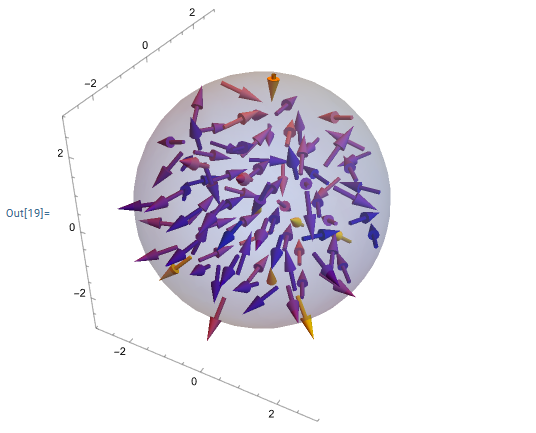
\includegraphics[width=0.75\linewidth]{image1.png}
\end{figure}
\newpage
\section*{Задача 2}
\subsubsection*{Получение решения}
Перепишем условие задачи:
$$\begin{cases}
    \Delta v=0,\\
    v|_{r=2}=4\sin(\varphi)\sin(\theta)\cos^2(\theta),\\
    v|_{r=5}=6\cos^2(\varphi)\sin^2(\theta)\cos(\theta).
\end{cases}$$
Решение этой задачи ищем в виде:
$$v(r,\varphi,\theta)=\sum_{n,m=0}^\infty (A_{nm}r^n+B_{nm}r^{-(n+1)})\cos(m\varphi)+(C_{nm}r^n+D_{nm}r^{-(n+1)})\sin(m\varphi))P_n^{(m)}(\cos(\theta)).$$
Подставим граничные условия:
$$v|_{r=2}=\sum_{n,m=0}^\infty (A_{nm}2^n+B_{nm}2^{-(n+1)})\cos(m\varphi)+(C_{nm}2^n+D_{nm}2^{-(n+1)})\sin(m\varphi))P_n^{(m)}(\cos(\theta))=$$$$=4\sin{\varphi}\sin{\theta}\cos^2{\theta}.$$
Отсюда,
$$\sum_{n=0}^\infty(C_{n1}2^n+D_{n1}2^{-(n+1)})P_n^{(1)}(\cos(\theta))=4\sin(\theta)\cos^2(\theta).$$
Введем замену $\cos(\theta)=x,$ тогда правая часть примет вид:
$$4x^2(1-x^2)^\frac{1}{2},\Rightarrow \deg(P_n^{(1)})\leq3.$$
Полиномы Лежандра для $n=\overline{1,3}$ мы уже использовали.
 Распишем правую часть через полиномы Лежандра:
 $$4\sin(\theta)\cos^2(\theta)=\frac{8}{15}P_3^{(1)}(\cos(\theta))+\frac{4}{5}P_1^{(1)}(\cos(\theta)).$$
 Подставим:
 $$(2C_{11}+2^{-2}D_{11})P_1^{(1)}(\cos(\theta))+(2^2C_{21}+2^{-3}D_{21})P_2^{(1)}(\cos(\theta))+(2^3C_{31}+2^{-4}D_{31}))P_3^{(1)}(\cos(\theta))=$$$$=\frac{8}{15}P_3^{(1)}(\cos(\theta))+\frac{4}{5}P_1^{(1)}(\cos(\theta)).$$
 Тогда получим систему:
 $$\begin{cases}
     2C_{11}+2^{-2}D_{11}=\frac{4}{5},\\
     2^2C_{21}+2^{-3}D_{21}=0,\\
     2^3C_{31}+2^{-4}D_{31}=\frac{8}{15}.
 \end{cases}$$
 Рассмотрим теперь второе граничное условие:
 $$v|_{r=5}=\sum_{n,m=0}^\infty (A_{nm}5^n+B_{nm}5^{-(n+1)})\cos(m\varphi)+(C_{nm}5^n+D_{nm}5^{-(n+1)})\sin(m\varphi))P_n^{(m)}(\cos(\theta))=$$
 $$=6\cos^2(\varphi)\sin^2(\theta)\cos(\theta)=3\sin^2(\theta)\cos(\theta)+3\cos(2\varphi)\sin^2(\theta)\cos(\theta).$$
 Таким образом, получаем два уравнения:
 $$\sum_{n=0}^\infty (A_{n0}5^n+B_{n0}5^{-(n+1)})P_n^{(0)}(\cos(\theta))=3\sin^2(\theta)\cos(\theta),$$
 $$\sum_{n=0}^\infty (A_{n2}5^n+B_{n2}5^{-(n+1)})P_n^{(2)}(\cos(\theta))=3\sin^2(\theta)\cos(\theta).$$
 Рассмотрим первое уравнение. Степень правой части по $\cos(\theta)$ равна 3, следовательно $\deg(P_n^{(0)})=n\leq3.$ Подставим $P_n^{(0)}, n=\overline{0,3}$ из первого задания:
 $$(A_{00}+B_{n0}5^{-1})P_0^{(0)}(\cos(\theta))+(A_{10}5+B_{10}5^{-2})P_1^{(0)}(\cos(\theta))+(A_{20}5^2+B_{20}5^{-3})P_2^{(0)}(\cos(\theta))+$$$$+(A_{30}5^3+B_{30}5^{-4})P_3^{(0)}(\cos(\theta))=\frac{6}{5}P_1^{(0)}(\cos(\theta))-\frac{6}{5}P_3^{(0)}(\cos(\theta)).$$
 Отсюда получаем систему:
 $$\begin{cases}
     A_{00}+B_{00}5^{-1}=0,\\
     A_{10}5+B_{10}5^{-2}=\frac{6}{5},\\
     A_{20}5^2+B_{20}5^{-3}=0,\\
     A_{30}5^3+B_{30}5^{-4}=-\frac{6}{5}.
 \end{cases}$$
 Рассмотрим второе уравнение, $\deg(P_n^{(2)})=n\leq3.$ Тоже воспользуемся прошлым заданием и сразу подставим:
 $$(A_{22}5^2+B_{22}5^{-3})P_2^{(2)}(\cos(\theta))+(A_{32}5^3+B_{32}5^{-4})P_3^{(2)}(\cos(\theta))=\frac{1}{5}P_3^{(2)}.$$
 Отсюда:
 $$\begin{cases}
     A_{22}5^2+B_{22}5^{-3}=0,\\
     A_{32}5^3+B_{32}5^{-4}=\frac{1}{5}.
 \end{cases}$$
 Для разрешения полученных систем возьмем недостающие уравнения из соседнего граничного условия, то есть для уравнений, полученных из второго граничного условия, возьмем уравнения, полученные из первого граничного условия и наоборот.
 $$\begin{cases}
     A_{10}5+B_{10}5^{-2}=\frac{6}{5},\\
     A_{10}2+B_{10}2^{-2}=0,
 \end{cases},\Rightarrow [\text{Wolfram Mathematica}], \Rightarrow
 \begin{cases}
     A_{10}=\frac{10}{39},\\
     B_{10}=-\frac{80}{39},
 \end{cases}$$
  $$\begin{cases}
     A_{30}5^3+B_{30}5^{-4}=-\frac{6}{5},\\
     A_{30}2^3+B_{30}2^{-4}=0,
 \end{cases},\Rightarrow [\text{Wolfram Mathematica}], \Rightarrow
 \begin{cases}
     A_{30}=-\frac{250}{25999},\\
     B_{30}=\frac{32000}{25999},
 \end{cases}$$
  $$\begin{cases}
     A_{32}5^3+B_{32}5^{-4}=\frac{1}{5},\\
     A_{32}2^3+B_{32}2^{-4}=0,
 \end{cases},\Rightarrow [\text{Wolfram Mathematica}], \Rightarrow
 \begin{cases}
     A_{32}=\frac{125}{77997},\\
     B_{32}=-\frac{16000}{77997},
 \end{cases}$$
  $$\begin{cases}
     C_{11}2+D_{11}2^{-2}=\frac{4}{5},\\
     C_{11}5+D_{11}5^{-3}=0,
 \end{cases},\Rightarrow [\text{Wolfram Mathematica}], \Rightarrow
 \begin{cases}
     C_{11}=-\frac{16}{585},\\
     D_{11}=\frac{400}{117},
 \end{cases}$$
  $$\begin{cases}
     C_{31}2^3+D_{31}2^{-4}=\frac{8}{15},\\
     C_{31}5^3+D_{31}5^{-4}=0,
 \end{cases},\Rightarrow [\text{Wolfram Mathematica}], \Rightarrow
 \begin{cases}
     C_{31}=-\frac{128}{1169955},\\
     D_{31}=\frac{2000000}{233991}.
 \end{cases}$$
 Таким образом, подставив получившиеся коэффициенты в полученные ранее представления, получим решение рассматриваемой задачи.
 $$v(r,\varphi, \theta)=\Big((\frac{10}{39}r-\frac{80}{39}r^{-2})P_1^{(0)}(\cos(\theta))+(-\frac{250}{25999}r^3+\frac{32000}{25999}r^{-4})P_3^{(0)}(\cos(\theta))\Big)\cos(0\varphi)+$$$$+\Big((\frac{125}{77997}r^3-\frac{16000}{77997}r^{-4})P_3^{(2)}(\cos(\theta))\Big)\cos(2\varphi)+$$$$+\Big((-\frac{16}{585}r+\frac{400}{117}r^{-2})P_1^{(1)}(\cos(\theta))+(-\frac{128}{1169955}r^3+\frac{2000000}{233991}r^{-4})P_3^{(1)}(\cos(\theta))\Big)\sin(\varphi)$$
\subsection*{Визуализация решения}
\begin{figure}
    \centering
    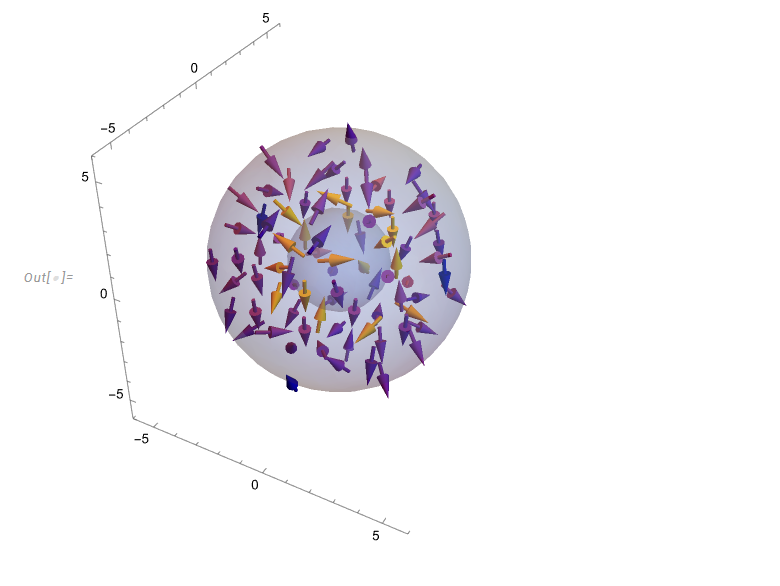
\includegraphics[width=1\linewidth]{image2.png}
\end{figure}
\end{document}
